\documentclass[10pt, conference, compsocconf]{IEEEtran}

% packages
\usepackage{algorithm}
\usepackage{algorithmic}
\usepackage{amsfonts} % for R symbol (the set of real numbers)
\usepackage{color}
\usepackage[pdftex]{graphicx}
\usepackage{graphicx}
\usepackage[bookmarks=false]{hyperref}
\hypersetup{colorlinks=true,linkcolor=black,citecolor=black,filecolor=black,urlcolor=blue}
\usepackage{mathtools}
\usepackage{multirow}
\usepackage{stmaryrd} % for llbracket and rrbracket
\usepackage{subcaption}
\usepackage{nicefrac}
\DeclarePairedDelimiter{\ceil}{\lceil}{\rceil}
\DeclarePairedDelimiter{\floor}{\lfloor}{\rfloor}

% new commands
\newcommand{\todo}[1]{\marginpar{\parbox{18mm}{\flushleft\tiny\color{red}\textbf{TODO}:
      #1}}}
\newcommand{\comment}[1]{\marginpar{\parbox{18mm}{\flushleft\tiny\color{blue}\textbf{Comment}:
      #1}}}

\newcommand{\note}[1]{
  \color{blue}\emph{[Note: #1]}
  \color{black}
}

\begin{document}

\title{Predicting computational reproducibility of scientific pipelines using collaborative filtering}

\author{Soudabeh Barghi, Lalet Scaria, Tristan Glatard\\
  Department of Computer Science and Software Engineering\\ Concordia University, Montreal, Quebec, Canada\\
  {first.last}@concordia.ca\\
  $^*$ These authors have contributed equally
}

\maketitle

\begin{abstract}
\end{abstract}


\section{Introduction}

Computational reproducibility, the property through which
computational results can be recomputed over time and
space~\cite{stodden}, has become a critical component of scientific
methodology with the rise of the reproducibility crisis in several
domains~\cite{xxx}. Among the factors hampering computational
reproducibility, infrastructural characteristics such as the operating
system play an important role. In neurosciences, our primary field of
interest, several studies have shown the effect of the operating
system on computational results. However, conducting such
reproducibility studies at scale is cumbersome due to the execution
time of data analysis pipelines, which easily exceeds a few hours.

In this paper we investigate approximate methods to predict the
reproducibility of a computational analysis from the first files that
it produces. Our main intuition is that reproducibility errors are
caused by a reduced number of factors that originate in the analysis
pipeline and input data. 

% Computational reproducibility is an issue, for instance among
% different operating systems (refer to Glatard FINF 2015,
% Gronenschild 2012).

% Scientific data analysis pipeline executions are long (give examples
% from neuroimaging).

% Refer to Germain et al 2008.

% Define subjects, pipelines.

% Problem: predict the reproducibility of pipeline files from other
% subjects and the first files produced by a pipeline. Restrict the
% study to binary classification.




\section{Method}

what is specific to our problem compared to regular collaborative filtering:
%+ subjects are equivalent to users. Not all subjects have the same input data. Anatomical variability, acquisition variability (e.g., 1 subject may have multiple T1s).
%+ files are produced in a specific order (movies aren't),
% which add constraints on the training set (cannot sample late files and not early ones).
%+ utility matrix is not sparse: we can potentially populate it completely. Which means that we can decide precisely which samples we need (active sampling). Therefore we can take the first row and first column to avoid cold start issues.

\subsection{Collaborative filtering using ALS}

We consider the collaborative filtering method as implemented in Spark's MLlb.
% Summarize Koren, Bell and Volinsky: https://dl.acm.org/citation.cfm?id=1608614

% Explain that you have binary classes (rounding)

% Biases


\subsection{Sampling the training set}

We investigated the following sampling techniques for the training set. 
In each method, we included the first row of the matrix (first 
generated file of each subject) and a random column (all files of a 
random subject) to avoid cold start issues. 

% 0. random unreal (baseline)
\paragraph{Random Unreal}
The training set is sampled randomly with no restriction, that is,
regardless of the file generation time. This method will be used as a
baseline for comparison with other methods, although it is not
realistic. Figure~\ref{fig:Random-Unreal-Sample-Training-set} represents 
a training set sampled using this method.


% 2. columns
\paragraph{Complete Columns}
The training set is sampled by randomly selecting complete columns in
the matrix, that is, complete subject executions. The last selected
column might be incomplete to meet the exact training ratio. This 
method is realistic: it corresponds to a situation where the 
collaborative filtering method will predict the reproducibility in the 
remaining subjects from the subjects in the training set. 
Figure~\ref{fig:Columns-Sample-Training-set} represents a training set 
sampled using this method.


% 3. rows
\paragraph{Complete Rows} The training set is sampled by selecting complete 
rows in the matrix, that is, the first files produced by
every execution. The last selected row might be incomplete to meet the
exact training ratio. This method is realistic: it corresponds to a 
situation where the processing of all the subjects is launched and 
interrupted before the execution is complete. The collaborative 
filtering method will then predict the reproducibility of the remaining 
files. Figure~\ref{fig:Rows-Sample-Training-set} represents a training 
set sampled using this method.
\begin{figure}[h!]
	\centering
	\begin{subfigure}[b]{0.4\linewidth}
		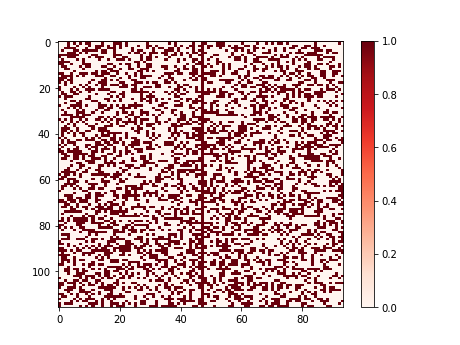
\includegraphics[width=\columnwidth]{figures/5vs7_random-unreal_04_training}
  		\caption{Random Unreal method}
  		\label{fig:Random-Unreal-Sample-Training-set}
	\end{subfigure}
	\begin{subfigure}[b]{0.4\linewidth}
  		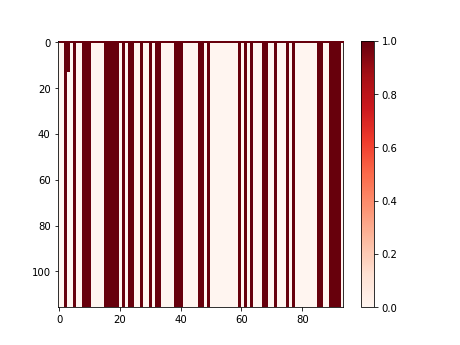
\includegraphics[width=\columnwidth]{figures/5vs7_columns_04_training}
  		\caption{Complete Columns method}
  		\label{fig:Columns-Sample-Training-set}
	\end{subfigure}
	\begin{subfigure}[b]{0.4\linewidth}
  		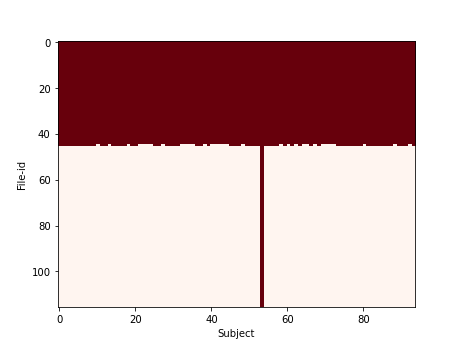
\includegraphics[width=\columnwidth]{figures/5vs7_rows_04_training}
  		\caption{Complete Rows method}
  		\label{fig:Rows-Sample-Training-set}
	\end{subfigure}
	\begin{subfigure}[b]{0.4\linewidth}
 		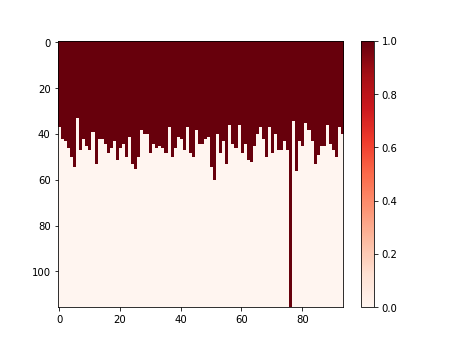
\includegraphics[width=\columnwidth]{figures/5vs7_random-real_04_training}
		\caption{Random Subjects method}
  		\label{fig:Uniform-S-Sample-Training-set}
	\end{subfigure}
	\begin{subfigure}[b]{0.4\linewidth}
  		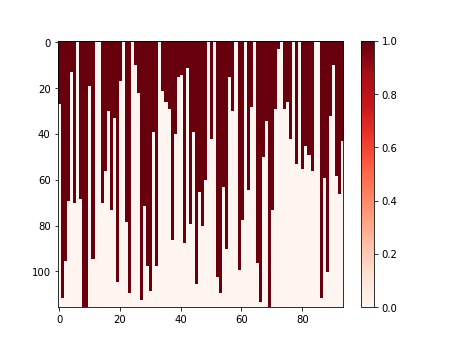
\includegraphics[width=\columnwidth]{figures/5vs7_diagonal_04_training}
  		\caption{(Uniform) method }
  		\label{fig:Diagonal-Sample-Training-set}
	\end{subfigure}
	\begin{subfigure}[b]{0.4\linewidth}
  		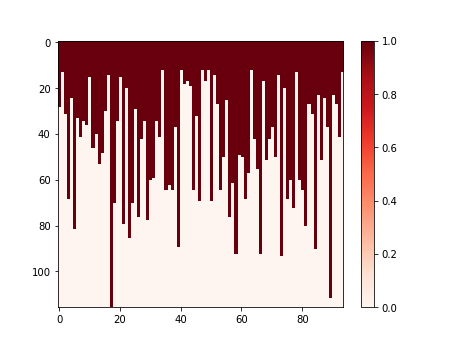
\includegraphics[width=\columnwidth]{figures/5vs7_random-triangular-largest_04_training}
  		\caption{(Triangular-L) method}
  		\label{fig:triangular-L-Sample-Training-set}
	\end{subfigure}
	\begin{subfigure}[b]{0.4\linewidth}
  		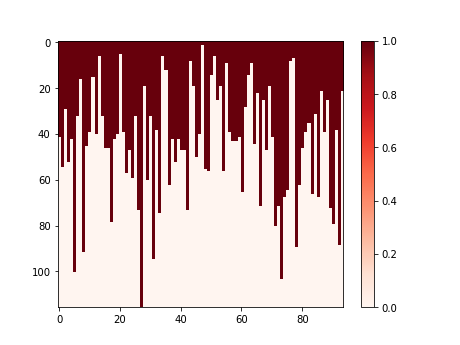
\includegraphics[width=\columnwidth]{figures/5vs7_random-triangular-smallest_04_training}
  		\caption{(Triangular-S) method}
  		\label{fig:triangular-S-Sample-Training-set}
	\end{subfigure}
	\caption{Sample training set for different methods with a training ratio of 0.4.}		
\end{figure}

\paragraph{Random Subjects -- RS} This method builds the 
training set by selecting the files from random subjects 
until the training ratio is reached. The file selected in a 
subject is the file with the lowest index in this subject that has not 
been already selected in the training set. This method is realistic as 
files are sampled according to their production time-stamps. 
Figure~\ref{fig:Uniform-S-Sample-Training-set} represents a training 
set sampled using this method.

\paragraph{Random File Numbers (Uniform) -- RFNU}

The number of files selected for every subject is randomly selected in
a uniform distribution $U(\textit{a},\textit{b})$, where \textit{b} is set to the total
number of files $N_{f}$ and \textit{a} is set according to training ratio $\alpha$ as follows:

\[
  \begin{cases}
          \textit{a} = 0      & \text{if $\alpha \leq 0.5$ }\\
          
          \textit{a} = (2\alpha - 1) N_{f} & \text{if $\alpha > 0.5$}
  \end{cases}
\]


This method is realistic as files are sampled according to their production time-stamps.
Due to sampling issues, it is possible that the actual training ratio obtained with this method
does not match the target one. We check that the difference between the target and real training ratios
was lower than 0.01.\\ 

\paragraph{Random File Numbers (Triangular) -- RFNT}
The number of files selected for every subject is randomly selected in
a triangular distribution with parameters \textit{a}, \textit{b} and 
\textit{c} (\todo{see Figure X}). The mean of the distribution is 
$\frac{a+b+c}{3}$. In our case, we set \textit{c} to $N_{f}$ and we set 
\textit{a} and \textit{b} with two approaches meant to ensure that the 
average of the distribution is $\alpha N_{f}$ ($\alpha$ is the training 
ratio):
\begin{enumerate}
        \item Largest a (RFNT-L): a is set to the 
        largest possible value, i.e., b. The average of the 
        distribution is $\frac{2a+N_{f}}{3}$, therefore 
        $a=\frac{3\alpha-1}{2}N_{f}$.
                \item Smallest a (RFNT-S): a is 
        set to the smallest possible value, i.e., 0. The average of the 
        distribution is $\frac{b+N_{f}}{3}$, therefore 
        $b=N_{f}(3\alpha-1)$. To ensure that $b<N_{f}$, we actually set 
        $b=\min(N_{f}, N_{f}(3\alpha-1))$. 
\end{enumerate}
It should be noted that $\alpha$ must be larger than $\frac{1}{3}$ for 
a and b to remain positive. For training ratios lower than $\frac{1}{3}$, we 
define RFNT methods as the RFNU one presented previously.

As illustrated in Figures~\ref{fig:triangular-L-Sample-Training-set} 
and~\ref{fig:triangular-S-Sample-Training-set}, the motivation for the 
RFNT-L method is to guarantee that, for large enough values of 
$\alpha$, all subjects will have at least a few files in the training 
set.

\section{Dataset}

We collected data to evaluate the computational reproducibility of analysis
pipelines of the Human Connectome Project~\cite{general-hcp}. We
processed a set S of 94 subjects randomly selected in the S500 HCP
release~\todo{URL} in three execution conditions with different
versions of the CentOS operating system (5.?, 6.? and 7.?), using the
PreFreesurfer, Freesurfer, PostFreesurfer and fMRIVolume pipelines
described in~\cite{hcp-pipelines} and available at \todo{URL}. For
each pipeline, we identified the set F of files produced for all
subjects in all conditions. For each condition pair and each pipeline,
we computed a binary difference matrix D of size $|F|\times|S|$, where $D_{i,j}$ is true
if file $i$ of subject $j$ was different in each condition. Rows of
$M$ are ordered by ascending file modification time in the pipeline.

Figure~\ref{fig:utility metrices} shows the difference matrices
obtained for the PreFreesurfer pipeline. The computational
reproducibility of the PreFreesurfer pipeline varies across subjects,
which motivates our study. Nevertheless, some files behave
consistently across all subjects, leading to complete black or white
lines. The ratio of positive elements in utility matrix of CentOS5 vs CentOS6(C5C6),  CentOS5 vs CentOS7(C5C7) and  CentOS6 vs CentOS7(C6C7) are
$0.34$, $0.79$ and $0.79$ respectively.

\begin{figure}[h!]
  \centering
  \begin{subfigure}[b]{0.5\linewidth}
	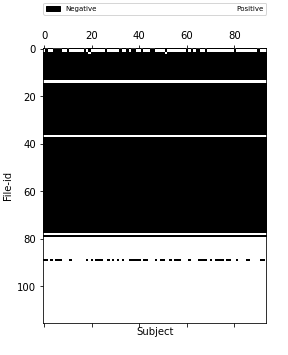
\includegraphics[width=\columnwidth]{figures/utility_5vs6_PFS}
  \caption{Utility matrix of CentOS5 vs CentOS6}
  \end{subfigure}
  \begin{subfigure}[b]{0.5\linewidth}
	 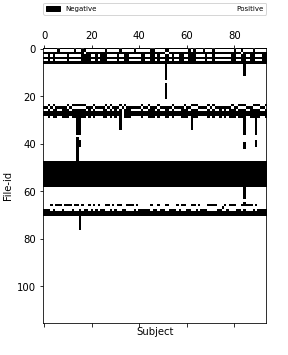
\includegraphics[width=\columnwidth]{figures/utility_5vs7_PFS}
  \caption{Utility matrix of CentOS5 vs CentOS7}
  \end{subfigure}
  \begin{subfigure}[b]{0.5\linewidth}
	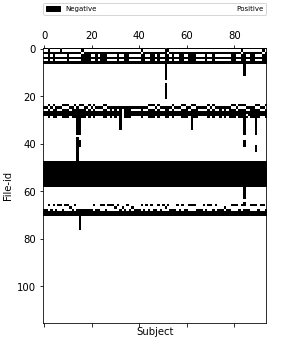
\includegraphics[width=\columnwidth]{figures/utility_6vs7_PFS}
  \caption{Utility matrix of CentOS6 vs CentOS7}
  \label{fig:utility metrices}
  \end{subfigure}
\end{figure}

as it can be seen, some of the files are consistent cross the subjects 
which means that there are some cases that a file has an error in whole subjects (complete white)or 
in another case no checksum difference has been observed for a file among all subjects (complete black).
These kind of consistent behaviour makes us to discard the prediction of these file-id's elements 
from the calculated accuracy in some phases of our experiments.      

% Describe your dataset: pipeline(s) used, input data, operating systems (CentOS5, 6, 7), matrix.

% 1. Prefreesurfer (what you have)
% 2. Freesurfer, with the same subjects as in Prefreesurfer.
% 3. PostFreesurfer
% 4. fmriVolume

\section{Results}


Four experiments have been conducted to evaluate the performance of our 
predictions using (1) ALS without biases, (2) ALS with biases, (3) Biases only. 
Results will be evaluated on the complete datasets and also specifically on the files that
do not behave consistently across subjects (\todo{explain this in introduction}).
\todo{the last sentence (pure accuracy) is just applied for Triangular-L, other results of ALS, ALS-biases are not applied in this case}
We evaluate prediction methods using accuracy, sensitivity and specificity defined as follows:
\[
        Accuracy = \frac{TP+TN}{TP+TN+FP+FN}
\]
\[
        Sensitivity = \frac{TP}{TP+FN}
\]
\[
        Specificity = \frac{TN}{TN+FP}
\]
Where TP is the number of True Positives (correctly predicted errors), 
FP is the number of False Positives, TN is the number of true negatives 
and FN is the number of false negatives.

We compare our methods to two references, (1) a dummy classifier that always predicts the dominant class.
as the dominant value of the utility matrix (1 or 0), (2) the Random Unreal method, used as the baseline sampling technique.

\subsection{ALS without biases}
In this phase of the experiment, the Alternating Least Squares 
technique of Collaborative Filtering is applied for all provided 
methods. Our four sampling techniques are compared in 
Figure~\ref{fig:ALS-Failure} and the results are described in the next 
sub-sections.

\begin{figure}[h!]
        \centering
        \begin{subfigure}[b]{0.8\linewidth}
                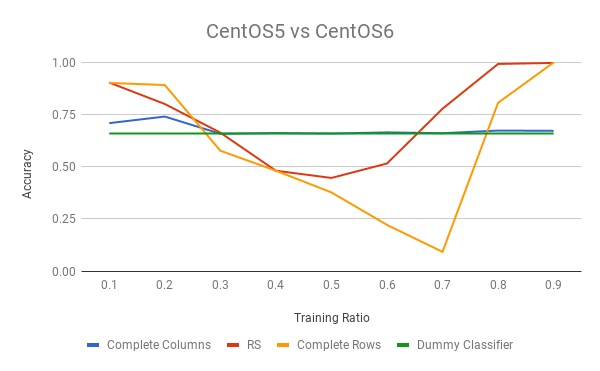
\includegraphics[width=\columnwidth]{figures/ALS/AlS-Failure-5vs6}
        \end{subfigure}
        \begin{subfigure}[b]{0.8\linewidth}
                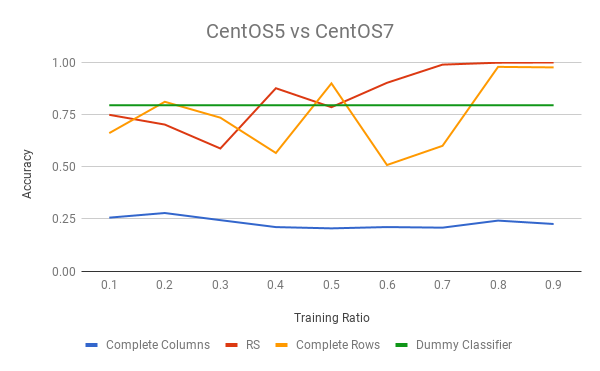
\includegraphics[width=\columnwidth]{figures/ALS/AlS-Failure-5vs7}
        \end{subfigure}
        \begin{subfigure}[b]{0.8\linewidth}
                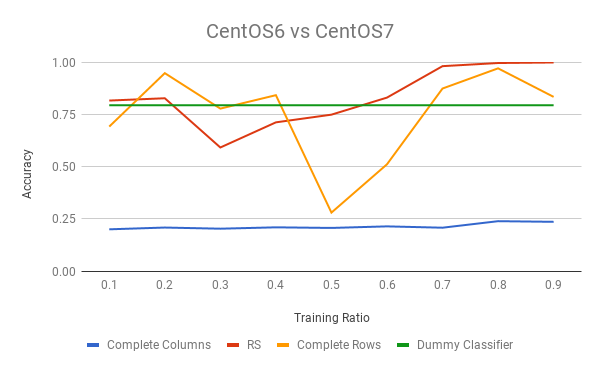
\includegraphics[width=\columnwidth]{figures/ALS/AlS-Failure-6vs7}
        \end{subfigure}
        \caption{Average accuracy of Complete Columns, RS, Complete Rows and Random Unreal methods in three different condition pairs.}
        \label{fig:ALS-Failure}
\end{figure}

\subsubsection{Random Unreal}
This method has a great performance with absolute accuracy of more than $0.95$ 
even by accessing to small training size of 10 percent. As it mentioned earlier 
this method is not applicable in pipeline due to time-stamp consideration but it 
is a good criterion to estimate the performance of other methods and try to modify 
the proposed methods in order to their accuracy be as closed as possible to the 
Random Unreal method ones.  


\subsubsection{Complete Columns}
The Complete Columns method has almost a constant accuracy even if the training ratio increased and it
is almost two times less than dummy classifier in more differentiated
condition pairs (CentOS5 vs CentOS7 and CentOS6 vs CentOS7). But in the
best case which it means in similar conditions the Complete Columns
accuracy is as much accurate as the Dummy classifier is, $0.65$
percent.
\\
\subsubsection{Complete Rows}
This method has some fluctuation over the gowth of training set size. These falactuations are more 
frequent in condition pairs which have higher difference positive ratio. 
Also by enlarging the training ratio specially between $0.3$ to $0.7$, 
we can see dummy classifier has better results than Complete Rows ones. 
In other words despite of better performance of Complete Rows than 
dummy classifier at the last 10 percent of the graph, its accuracy 
are less than dummy classifiers ones.  
\\
\subsubsection{Random Subjects-RS}
Same to the Complete Row method, RS method has some fluctuation but not as frequent 
as Complete Rows method. Although there are some up and down trends specially with 
training ratio range of $0.2$ to $0.6$ but its constant growth trend after 
training ratio $0.3$ in condition pairs with high difference positive ratio is considerable.
The method can be $0.99$ percent accurate when it has over 70 percent of the data however 
this accuracy can be achived with higher training ratio (over 80 percent) for C5C6.  
\\
\\
\noindent Figure~\ref{fig:ALS-Succeed} represents
the accuracy graph of all Random kind methods with comparison to dummy
classifier over the increment of the training ratio.\\
\begin{figure}[h!]
        \centering
        \begin{subfigure}[b]{0.8\linewidth}
                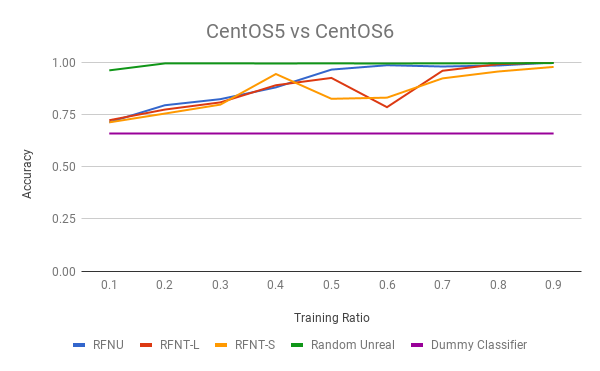
\includegraphics[width=\columnwidth]{figures/ALS/ALS-Succeed-5vs6}
        \end{subfigure}
        \begin{subfigure}[b]{0.8\linewidth}
                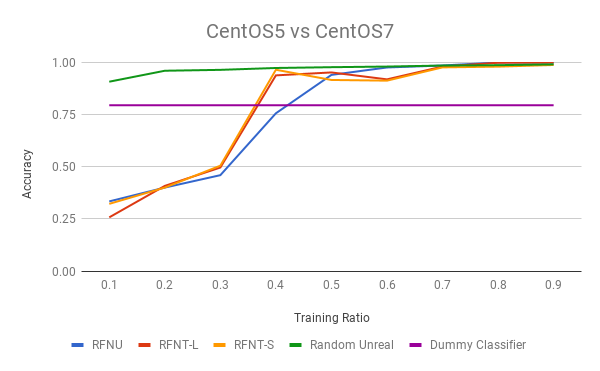
\includegraphics[width=\columnwidth]{figures/ALS/ALS-Succeed-5vs7}
        \end{subfigure}
        \begin{subfigure}[b]{0.8\linewidth}
                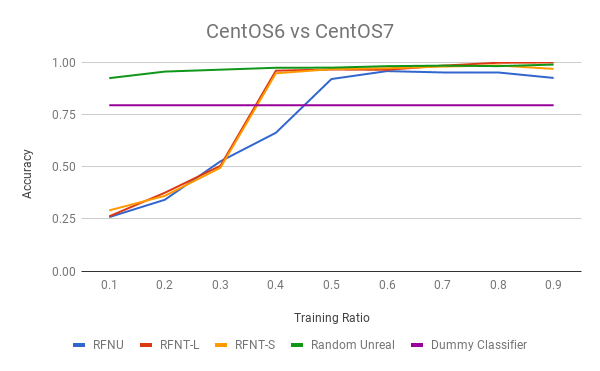
\includegraphics[width=\columnwidth]{figures/ALS/ALS-Succeed-6vs7}
        \end{subfigure}
        \caption{Average performance of RFNU methods in three different condition pairs}
        \label{fig:ALS-Succeed}
\end{figure}
\subsubsection{Random File Numbers(Uniform) - RFNU}
The continuous rise of RFNU accuracy trend can be observed in Figure~\ref{fig:ALS-Succeed}.
However a 0.03 drop is recorded in C6C7 between training ratio size of $0.8$ to $0.9$. 
This method takes over the dummy accuracy after having a training size more than 40 percent 
in condition pairs of C5vsC7 and C6vsC7 but it always shows better accuracy than 
dummy classifier ($0.73$ percent with training ratio of $0.1$).\newline

% ALS-RFNT approaches
\indent As it mentioned earlier, for $\alpha < \nicefrac{1}{3}$ RFNT approaches are not applicable, 
therefor for training ratio less than $0.4$ RFNU method is employed. As a result, in terms of 
evaluating the performance of RFNT-L and RFNT-S approches, only those accuracy results are 
considered which their training set are equal or greater than 0.4 percent of the whole utility matrix.\newline 

\subsubsection{RFNT-L}

In Figure~\ref{fig:ALS-Succeed}, the results show that RFNT-L performance is always more accurate than
dummy classifier even in its lowest accuracy value observed at training ratio of $0.6$ in C5C6 ($0.78$ percent).
Despite of this sudden, RFNT-L method has slight growing trend throughout the 
increment of training ratio and its accuracy is always more than $90\%$. 

\subsubsection{RFNT-S}
Figure~\ref{fig:ALS-Succeed} shows the overall performance of RFNT-S methods in three different condition pairs.
Similar to RFNT-L, this method also has constant accuracy increment with maximum less accuracy of 0.07 than 
Random Unreal method throughout the experiment of C5C7 and C6C7.

%%%%%%%%%%%%%%%%%%%%%%%%%%%%%%%%%%%%%%%%%%
\subsection{ALS with biases}
In this part of the experiment, the effect of both subject and file 
biases are considered in the prediction. Our three random sampling 
techniques (RFNU, RFNT-L and RFNT-S) are compared in 
Figure~\ref{fig:ALS-Bias-PFS} as a function of the training 
ratio $\alpha$.

\begin{figure}[h!]
        \centering
        \begin{subfigure}[b]{0.8\linewidth}
                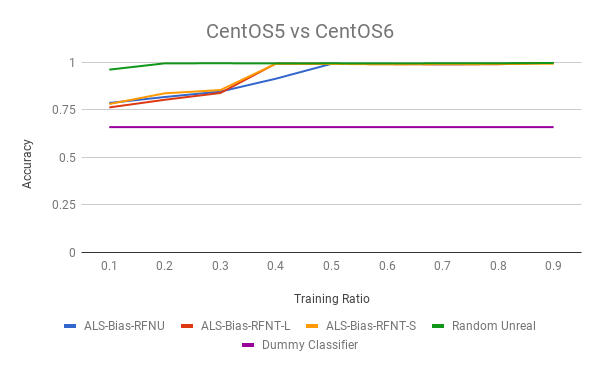
\includegraphics[width=\columnwidth]{figures/ALS-Bias/ALS-Bias-5vs6-PFS}
        \end{subfigure}
        \begin{subfigure}[b]{0.8\linewidth}
                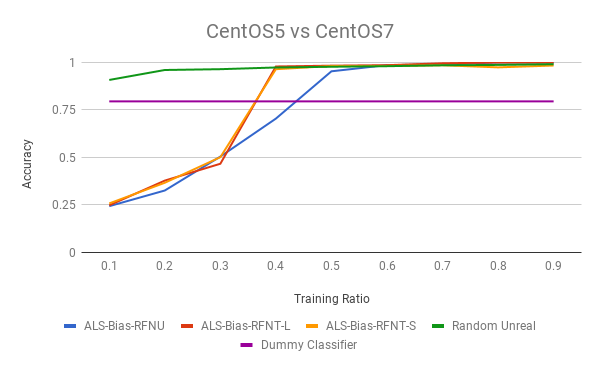
\includegraphics[width=\columnwidth]{figures/ALS-Bias/ALS-Bias-5vs7-PFS}
        \end{subfigure}
        \begin{subfigure}[b]{0.8\linewidth}
                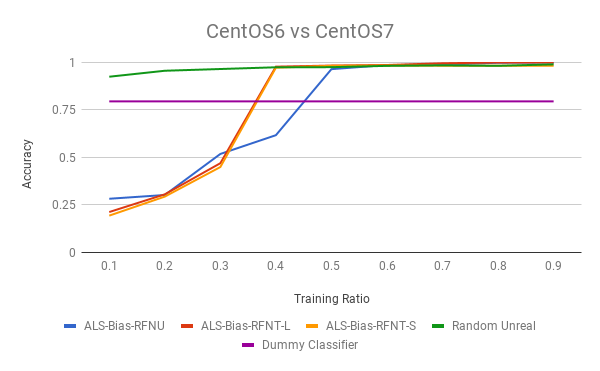
\includegraphics[width=\columnwidth]{figures/ALS-Bias/ALS-Bias-6vs7-PFS}
        \end{subfigure}
        \caption{Average performance of random methods for three different condition pairs (ALS with Bias).}
        \label{fig:ALS-Bias-PFS}
\end{figure}
\todo{Add $\alpha$ to the x labels in the Figure}

All three methods reach the accuracy of the baseline Random Unreal 
method from $\alpha$=0.5. RFNT methods reach this accuracy earlier than 
RFNU, from $\alpha$=0.4. For lower training ratios, all methods 
outperform the dummy classifier for one condition pair (CentOS5 vs 
CentOS6) but this is not the case for the other conditions. It should 
be noted that, as explained before, the three methods boil down to the 
same one (RFNU) for $\alpha<$0.3.{}
%%%%%%%%%%%%%%%%%%%%%%%%%%%%%%%%%%%%%%%%%%%%%%%%%%%
\subsection{Bias without ALS}
In this part of our experiments we tried to eliminate the ALS prediction 
impact on the results therefore, the elements of the matrix are going to 
be predicted according to the biases of both their constitutive subject and file-id.
Figure~\ref{fig:Bias-PFS} represents
the accuracy graph of all methods as a function of the training ratio in Biases without ALS technique. 
\begin{figure}[h!]
        \centering
        \begin{subfigure}[b]{0.8\linewidth}
                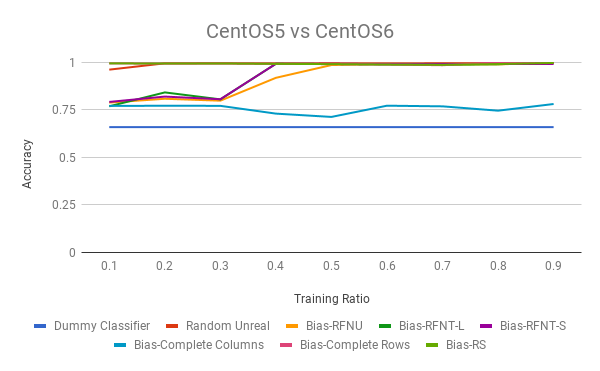
\includegraphics[width=\columnwidth]{figures/Bias/Bias-5vs6-PFS}
        \end{subfigure}	
        \begin{subfigure}[b]{0.8\linewidth}
                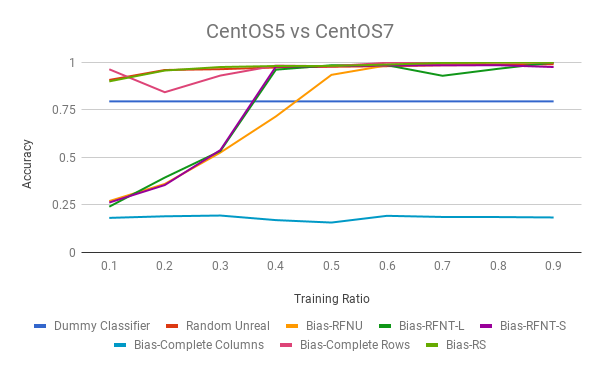
\includegraphics[width=\columnwidth]{figures/Bias/Bias-5vs7-PFS}
        \end{subfigure}
        \begin{subfigure}[b]{0.8\linewidth}
                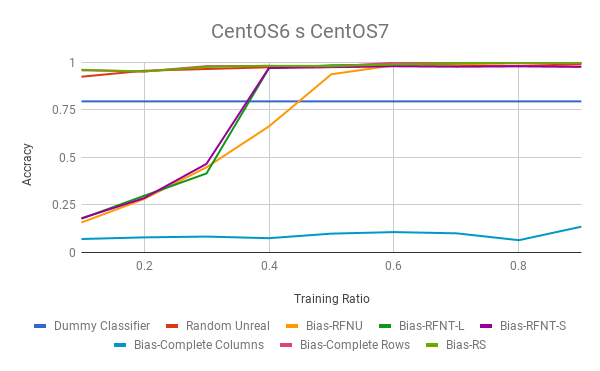
\includegraphics[width=\columnwidth]{figures/Bias/Bias-6vs7-PFS}
        \end{subfigure}
        \caption{Average performance of all methods for three different condition pairs (Bias without ALS).}
        \label{fig:Bias-PFS}
\end{figure}

As it can be seen, Complete Columns method is less accurate than dummy classifier
 with less than 25 percent accuracy but this is not the case for the CentOS5 vs CentOS6 
 condition pair which it outperform dummy classifier (with accuracy of 75).
Despite of inadequate accuracy of RS and Complete Rows sampling methods in ALS without Biases prediction technique,
 they surpass other methods with the same accuracy of the baseline Random Unreal method.
Triangular Distribution methods(RFNT-L, RFNT-S) reach to the baseline accuracy by $\alpha$=0.4, 
which is earlier than the same happens for RFNU  by $\alpha$>0.5.{}
In general, all methods except complete columns have high accuracy almost as accurat as the Random Unreal baseline method
in this technique of prediction.As usual, three distributional methods perform equally by the only significant 
difference at $\alpha$=0.4{}.  


 
%%%%%%%%%%%%%%%%%%%%%%%%%%%%%%%%%%%%%%%%%%%%%%%%%%%
% General conclution on results of ALS without Bias 
%~ In general the accuracy pattern of the two Complete Rows and 
%~ RS methods show similar decline and grow behaviour over the 
%~ training ratio axis however it can be subject to considerable 
%~ fluctuations in differentiated condition pairs. Despite of their 
%~ likely irrational behaviour, they always have better accuracy 
%~ for the training size with less than $0.3$ in comparison to other 
%~ methods. This better performance (around 75 percent)is almost three 
%~ times higher than other methods in condition pairs with more 
%~ differences but just 20 percent better when the conditions are more 
%~ similar to each other (CentOS5 vs CentOS6) with accuracy of $90\%$.
%~ Figure~\ref{fig:RS_Rows} represents
%~ the accuracy graph of these two methods with comparison to dummy
%~ classifier over the increment of the training ratio.
%~ \begin{figure}[h!]
        %~ \centering
        %~ \begin{subfigure}[b]{0.4\linewidth}
                %~ 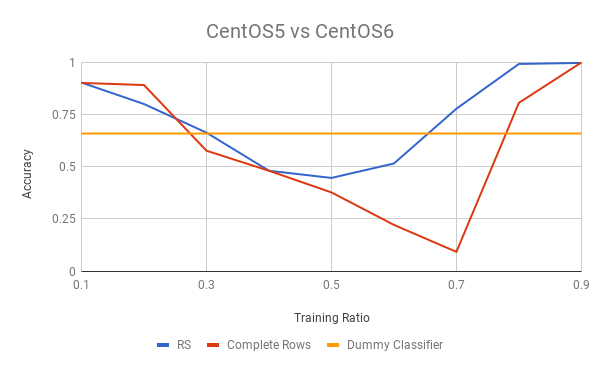
\includegraphics[width=\columnwidth]{figures/RS_Rows_5vs6}
        %~ \end{subfigure}
        %~ \begin{subfigure}[b]{0.4\linewidth}
                %~ 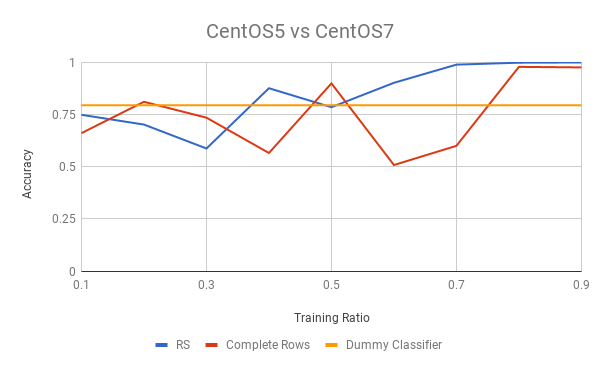
\includegraphics[width=\columnwidth]{figures/RS_Rows_5vs7}
        %~ \end{subfigure}
        %~ \begin{subfigure}[b]{0.4\linewidth}
                %~ 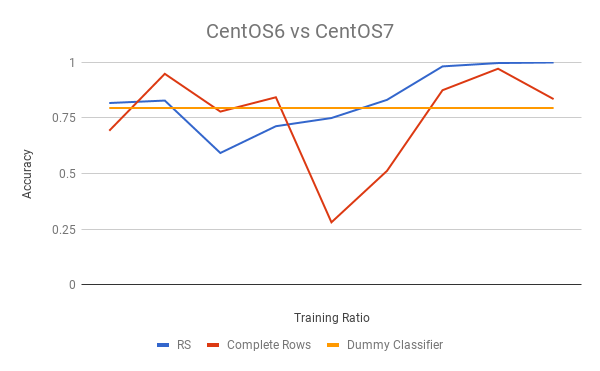
\includegraphics[width=\columnwidth]{figures/RS_Rows_6vs7}
        %~ \end{subfigure}
        %~ \caption{Average performance of RS and Complete Rows methods in three different condition pairs}
        %~ \label{fig:RS_RowS}
%~ \end{figure}

%~ All the other random methods, RS and both RFNT approaches 
%~ are performing a continues growth Figure~\ref{fig:simple-methods} represents
%~ the accuracy graph of all random methods with comparison to dummy
%~ classifier over the increment of the training ratio.. Although some considerable variation 
%~ for both triangular approaches have been observed (CentOS5 vs CentOS6) 
%~ their constant rise leads us to the next phase of experiments which was 
%~ adding up bias into the current ALS technique. 
%~ The training set suffers from lacking the files which are almost generated towards the end of pipeline.

%~ \begin{figure}[h!]
        %~ \centering
        %~ \begin{subfigure}[b]{0.4\linewidth}
                %~ 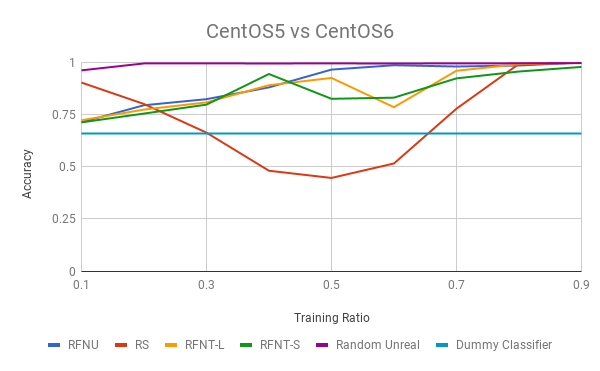
\includegraphics[width=\columnwidth]{figures/simple-methods-5vs6}
        %~ \end{subfigure}
        %~ \begin{subfigure}[b]{0.4\linewidth}
		%~ 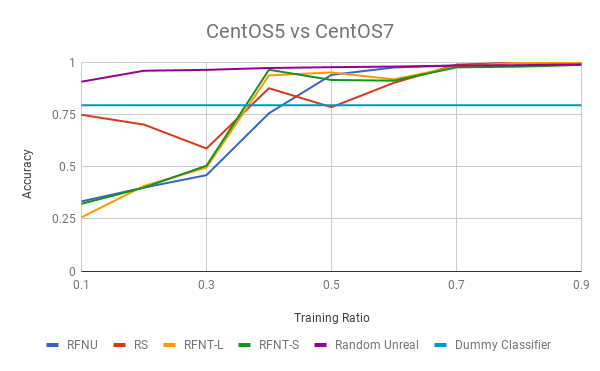
\includegraphics[width=\columnwidth]{figures/simple-methods-5vs7}
        %~ \end{subfigure}
        %~ \begin{subfigure}[b]{0.4\linewidth}
                %~ 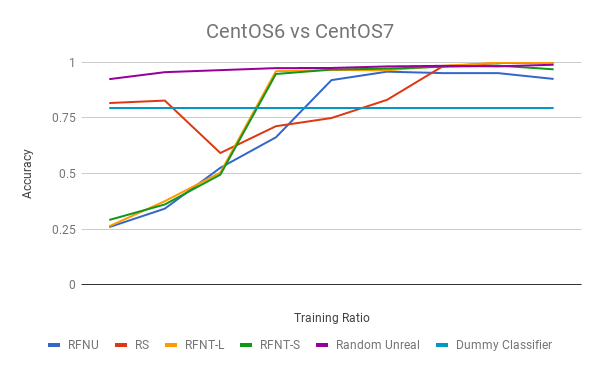
\includegraphics[width=\columnwidth]{figures/simple-methods-6vs7}
        %~ \end{subfigure}
	%~ \caption{Average performance of all methods in three different condition pairs}
	%~ \label{fig:simple-methods}
%~ \end{figure}





%-----------------------------------------------------------
% Present your results: accuracy, ROC curves, transparency matrix, factors. 

% Try with different numbers of factors. 

\section{Discussion}
this is just a test of compiling 

% Not all subjects behave the same, which motivates the Big Data approach. 

% Which sampling method is best

% Interpreting the factors? Factors reflect the pipeline definition. 

% How can this be used in practice

% What are the limitations

\section{Conclusion}

% Summary of the results and discussion. The take-home message.
%%%%%% why there is a drop in ALS-RFNT-L with 60% ratio?  
\section*{Acknowledgement}

\bibliographystyle{IEEEtran}
\bibliography{IEEEabrv,biblio.bib}


\end{document}
